\documentclass[12pt]{article}
\usepackage[paper=letterpaper, left=1in, right=1in, top=1in, bottom=1in]{geometry}

\usepackage[parfill]{parskip}
\usepackage{amsmath}
\usepackage{graphicx}

\begin{document}
\thispagestyle{empty}

\begin{center}
{\large CS 310}\\
Assignment 205
\end{center}

\begin{flushright}
Hieu Le
\end{flushright}

\textbf{Problem 1.} Algorithm A performs $10n^2$ basic operations, and
algorithm B performs $300\lg(n)$ basic operations. Which algorithm is
better, and at what value of n does the better algorithm start to show
its better performance? Illustrate your answer with a graph generated
by a program such as gnuplot or wolfram alpha.

\textit{Answer:} As depicted in the following graph:

\begin{center}
\scalebox{.4}{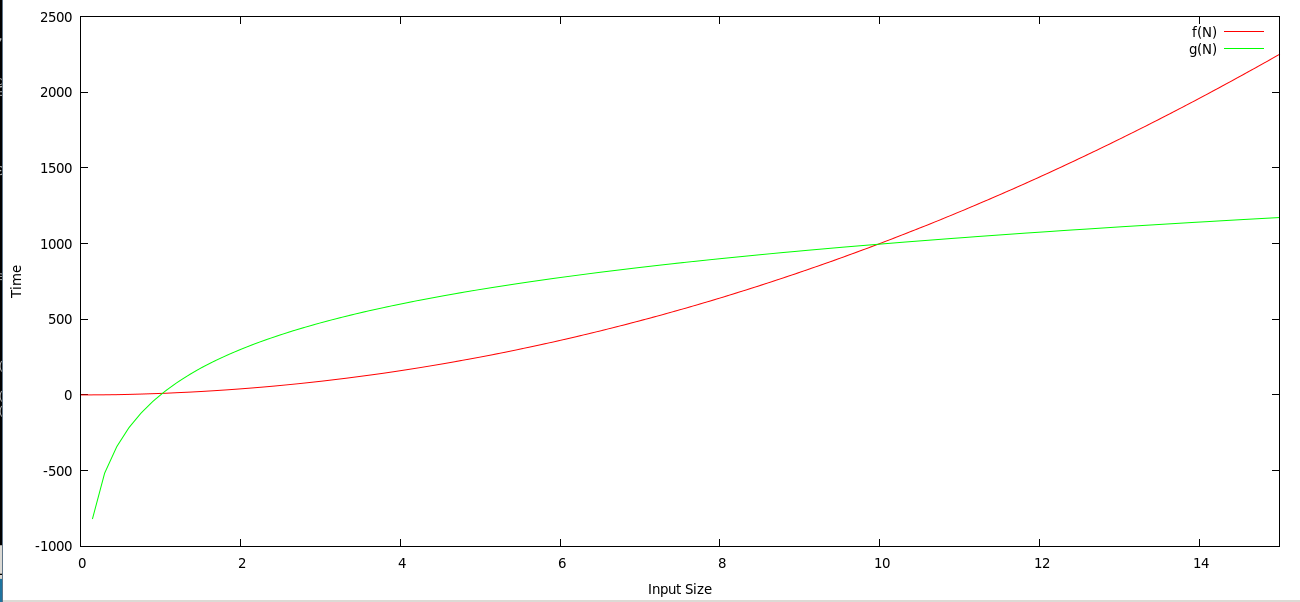
\includegraphics{plot.jpeg}}
\end{center}

Algorithm B is better than algorithm A. Algorithm B begins to show superior performance at $n = 10$.

\textbf{Problem 2.} Using the definitions,
show that
\[
6n^2 + 20n \in O(n^3)
\]
but
\[
6n^2 + 20n \not\in \Omega(n^3)
\]

\textit{Answer:} \\
Let $c = 30$ and $n_0 = 1$. Since $6n^2 + 20n \leq cn^3$ for all $n \geq n_0$, $6n^2 + 20n \in O(n^3)$.\\
Since $6n^2 + 20n$ is of smaller degree than $n^3$, $6n^2 + 20n$ is asymptotically smaller than $n^3$. Subsequently, there does not exist any pair of positive numbers $c$ and $n_0$ such that $6n^2 + 20n \geq cn^3$ for all $n \geq n_0$. Hence, $6n^2 + 20n \not\in \Omega(n^3)$.

\textbf{Problem 3.} Given the following algorithm, and assuming that $n$ is an even
        number, calculate the exact number of times
            statement \texttt{foo} runs, and analyze the algorithm
            using the the rules (e.g., polynomial).

\begin{verbatim}
j = 1;
while( j <= n/2 )
{
   i = 1;
   while( i <= j )
   {
      foo;
      i++;
   }
   j++;
}
\end{verbatim}


\textit{Answer:} \\
The number of times statement \texttt{foo} runs is:

\begin{align*}
T(n) &= \sum\limits_{j=1}^{n/2}(\sum\limits_{i=1}^j 1) = \sum\limits_{j=1}^{n/2} j  \\
&= 1 + 2 + 3 + ... + n/2 \\
&= (1 + n/2)(n/2)/2 \\
&= (2n + n^2)/8
\end{align*}

Since $(2n + n^2)/8$ is a polynomial of degree 2, $(2n + n^2)/8 \in \Theta(n^2)$. 


\textbf{Problem 4.} Solve the recurrence relation $t_n = 2nt_{n - 1}$
  where $t_0 = 1$.

\textit{Answer:} Using the given relation, we have:

\begin{align*}
t_n  &= 2nt_{n - 1} \\
     &= 2n(2(n - 1)t_{n - 2}) \\
     &= 2^2n(n - 1)t_{n - 2} \\
     &= 2^{n - (n - 2)} \times n!/(n - 2)! \times t_{n - 2} \\
     &= 2^{n - (n - 2)} \times n!/(n - 2)! \times (2(n - 2)t_{n - 3}) \\
     &= 2^{n - (n - 3)} \times n!/(n - 3)! \times t_{n - 3} \\
     & \vdots \\
     &= 2^{n - (n - k)} \times n!/(n - k)! \times t_{n - k} \\
     & \vdots \\
     &= 2^{n - (n - n)} \times n!/(n - n)! \times t_{n - n} \\
     &= 2^n n! t_0
\end{align*}
and therefore $t_n = 2^nn!$ for $n \geq 1$.

\textbf{Problem 5.} Analyze a program whose time complexity is $T(n) =
7T(\frac{n}{4}) + n$.

\textit{Answer:} \\
Applying the Master Theorem, we have: $a = 7, b = 4, d = 1$. \\
Since $a > b^d$, $T(n) \in \Theta(n^{log_47}) \approx \Theta(n^{1.404})$. 

\end{document}
